\chapter{Introduction}
Because RS485 is a half-duplex protocol, software on both ends of the physical data line should follow the same set of rules defined in the protocol and Message Format (see Chapter \ref{ch:message_format}). The Bus Manager is responsible for transferring commands and data between subsystems while adhering to this format.
This implies checking for CRC errors and sending a retransmission request or NACK when it needs to do so.
The Bus Manager acts between the Application Layer and the Physical Layer of the OSI model.

Figure \ref{fig:rs485_diagram} shows that there are 5 different RS485 buses inside the rover.
The Bus Manager also prevents any race condition on its assigned bus and makes sure that multiple apps cannot communicate with their subsystem at the same time.
\todo[inline]{Not sure about this yet}

\begin{figure}[H]
    \centering
    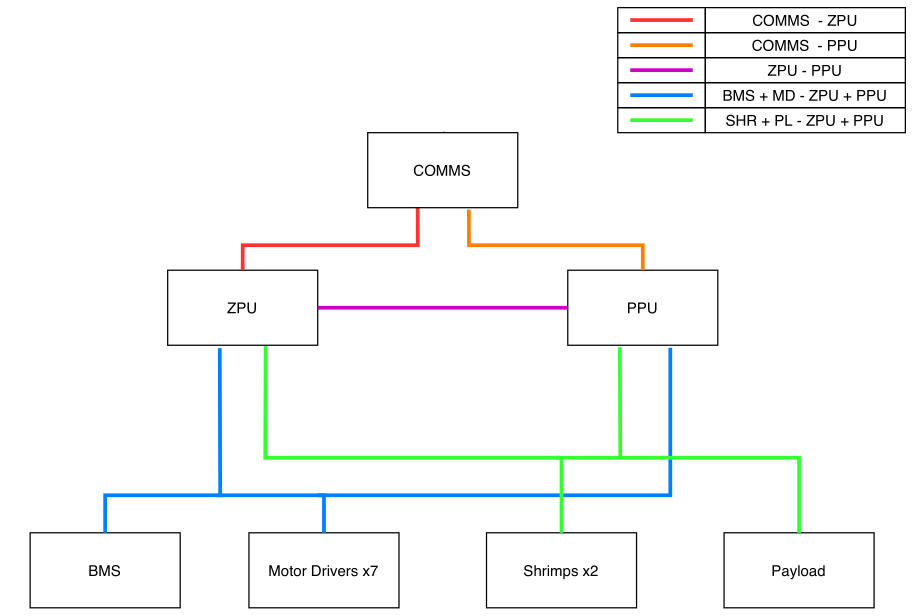
\includegraphics[scale=0.4]{figures/RS485_connections.png}
    \caption{Schematic view of the physical RS485 busses layout}
    \label{fig:rs485_diagram}
\end{figure}


\newpage


It is a bit awkward and impractical to uniquely identify RS485 buses based on the colours used in Figure \ref{fig:rs485_diagram}.
This is why we map the colours of Figure \ref{fig:rs485_diagram} to a unique bus name and number.
Table \ref{tab:buslegend} shows this mapping.
From now on in this document as well as in code, we will refer to bus names rather than bus colours.

\definecolor{amethyst}{rgb}{0.6, 0.4, 0.8}
\definecolor{bleudefrance}{rgb}{0.19, 0.55, 0.91}

\begin{longtable}{| p{0.1\textwidth} | p{0.15\textwidth} | }
    \hline
    \textcolor{red}{Bus name} & \textcolor{red}{Bus colour} \\
    \hline
    Bus0 & 
\begin{tikzpicture} \draw[line width=1mm, color=red] (0,0) -- (2,0); \end{tikzpicture} \\
    \hline
    Bus1 & 
\begin{tikzpicture} \draw[line width=1mm, color=orange] (0,0) -- (2,0); \end{tikzpicture} \\
    \hline
    Bus2 & 
\begin{tikzpicture} \draw[line width=1mm, color=amethyst] (0,0) -- (2,0); \end{tikzpicture} \\
    \hline
    Bus3 & 
\begin{tikzpicture} \draw[line width=1mm, color=bleudefrance] (0,0) -- (2,0); \end{tikzpicture} \\
    \hline
    Bus4 & 
\begin{tikzpicture} \draw[line width=1mm, color=green] (0,0) -- (2,0); \end{tikzpicture} \\
    \hline

    \caption{Bus legend mapping bus names to colours}
    \label{tab:buslegend}
\end{longtable}


\section{Background information and History}

\subsection{First version (1.0)}
Bus Manager is a concept that was first introduced in February 2021 as part of Max' thesis \cite{comms_thesis}.
Between February 2021 and August of 2021, the foundational layer of Bus Manager was laid which includes, but is not limited to, the Message Format.
Unit tests have shown that this first revision of Bus Manager used to work.

\subsection{Second version (2.0)}
In the second revision of Bus Manager, a few modifications have been made.
One of these changes is, for instance, that the Bus Manager won't send an initial message to request if an $x$ amount of bytes are available for the receiver to receive. Instead, it will just send the command which includes the length as part of the Message Format.
\todo[inline]{Clear up this sentence}
\par The second revision also uses a semaphore to synchronise bus access between bus managers, because the idea was for each subsystem app to have its own bus manager.

\subsection{Third version (2.1)}
The third version of the Bus Manager uses a more centralised approach. The Bus Managers live on the OBC in their own app, which coordinates bus access for all buses. Apps need to communicate with the Bus Managers via inter-thread communication. This avoids the need for using shared semaphores and decreases the dependencies between the subsystem apps. For further information about the design, see Chapter \ref{ch:design}.


\section{List of features of Bus Manager 2.1}

Now that the reader is aware of the overall functionality of the Bus Manager, we can list a set of features that characterises Bus Manager 2.1 (subject to change).

\begin{itemize}

    \item{\textbf{Instances}. Each bus has a separate instance of the Bus Manager that manages the access to that bus. Avoids the need for a more complex solution for all buses.}

    \item{\textbf{Timeout}. When a Bus Manager sends any type of message it waits for a response. A configurable timeout limit can be set to signal an error if the response is not received within that limit. }

    \item{\textbf{Retries}. When too many timeouts have happened and \textbf{<tbd>} retries are exceeded, then the application layer of this particular Bus Manager is informed about the failure.}

    \item{\textbf{Portability}. Because of the extensive use of Bus Manager both on the masters (OBC, PPU) and slaves (subsystems), it is of extra interest to design and implement Bus Mananger in such a way that it is easy to port over to subsystems which run different hardware architectures. Reimplementing it means that subsystem designers need to be fully aware of the protocol- and Message Format and this is a source of error and requires extra testing and validating. Bus Manager should be easily portable and be abstract in nature.}

    \item{\textbf{Sustainability}. Bus Manager shall comply to the Lunar Zebro Software guidelines. These include, but are not limited to: the code style guide and GoogleTest Unit Tests. The Git repository follows the same skeleton as all the other software modules.}

\end{itemize}
